\section{Akteure}

\centering
\begin{longtable}[c]{|p{2cm}|p{6cm}|p{6cm}|}
    \caption{Beschreibung der Akteure}
    \label{fig:akteur-tabelle}
    \endlastfoot
    \hline \multicolumn{3}{|r|}{{Weitergeführt auf der folgenden Seite}}                                                                                                                                                                             \\ \hline
    \endfoot
    \hline
    \endhead
    \hline
    \textbf{Akteur} & \textbf{Beschreibung}                                                                                                                                                                   & \textbf{Verwendet in Anwendungsfall} \\ \hline
    AppUser         & Greift auf Funktionen der App mit seinem Benutzer-Account zu. Je nach Rolle kann er den Status sowie dokumentierende Fotos und Kommentare von Leistungspositionen einsehen und \"andern &
    \begin{enumerate}
        \item Add documenting photo
        \item Change billing item status
        \item Display billing item status
        \item Push local changes to web server
    \end{enumerate}                                                                                                                                                                                                                        \\ \hline
    WebServer       & Hauptzugriffsstelle f\"ur alle vertrags- und projektrelevanten Daten. Dies ist kein menschlicher Akteur, sondern die Applikation, die die Funktionalität des Webservers bietet          &
    \begin{enumerate}
        \item Push local changes to web server
        \item Authenticate
    \end{enumerate}                                                                                                                                                                                                                        \\ \hline
    OrgAdmin        & Registriert Benutzer und legt Benutzerrollen fest für seine jeweilige Organisation                                                                                                      &
    \begin{enumerate}
        \item Remove org user
        \item Change role of org user
        \item Add org user
        \item Diagram: Plot states of billing items from one contract
        \item Configure diagrams
        \item Diagram: Plot construction progress
    \end{enumerate}                                                                                                                                                                                                                        \\ \hline
    SysAdmin        & F\"ugt Organisationen hinzu und bestimmt den Organisations-Admin einer Organisation                                                                                                     &
    \begin{enumerate}
        \item Add organization
        \item Assign org admin
        \item Configure diagrams
        \item Diagram: Plot construction progress
        \item Diagram: Plot states of billing items from one contract
        \item Diagram: Plot states of billing items from many contracts
    \end{enumerate}                                                                                                                                                                                                                        \\ \hline
    WebUser         & Verwendet die Nutzeroberfl\"ache des Webservers um Daten (auch Diagramme) einzusehen,  Status\"anderungen einzelner Leistungspositionen durchzuf\"uhren und Diagramme zu erstellen      &
    \begin{enumerate}
        \item Change status of position
        \item View organization's contracts
        \item Diagram: Plot states of billing items from one contract
        \item Diagram: Plot construction progress
    \end{enumerate}                                                                                                                                                                                                                        \\\hline
\end{longtable}

\newpage

\section{Anwendungsfalldiagramm - App}

\begin{figure}[h]
    \centering
    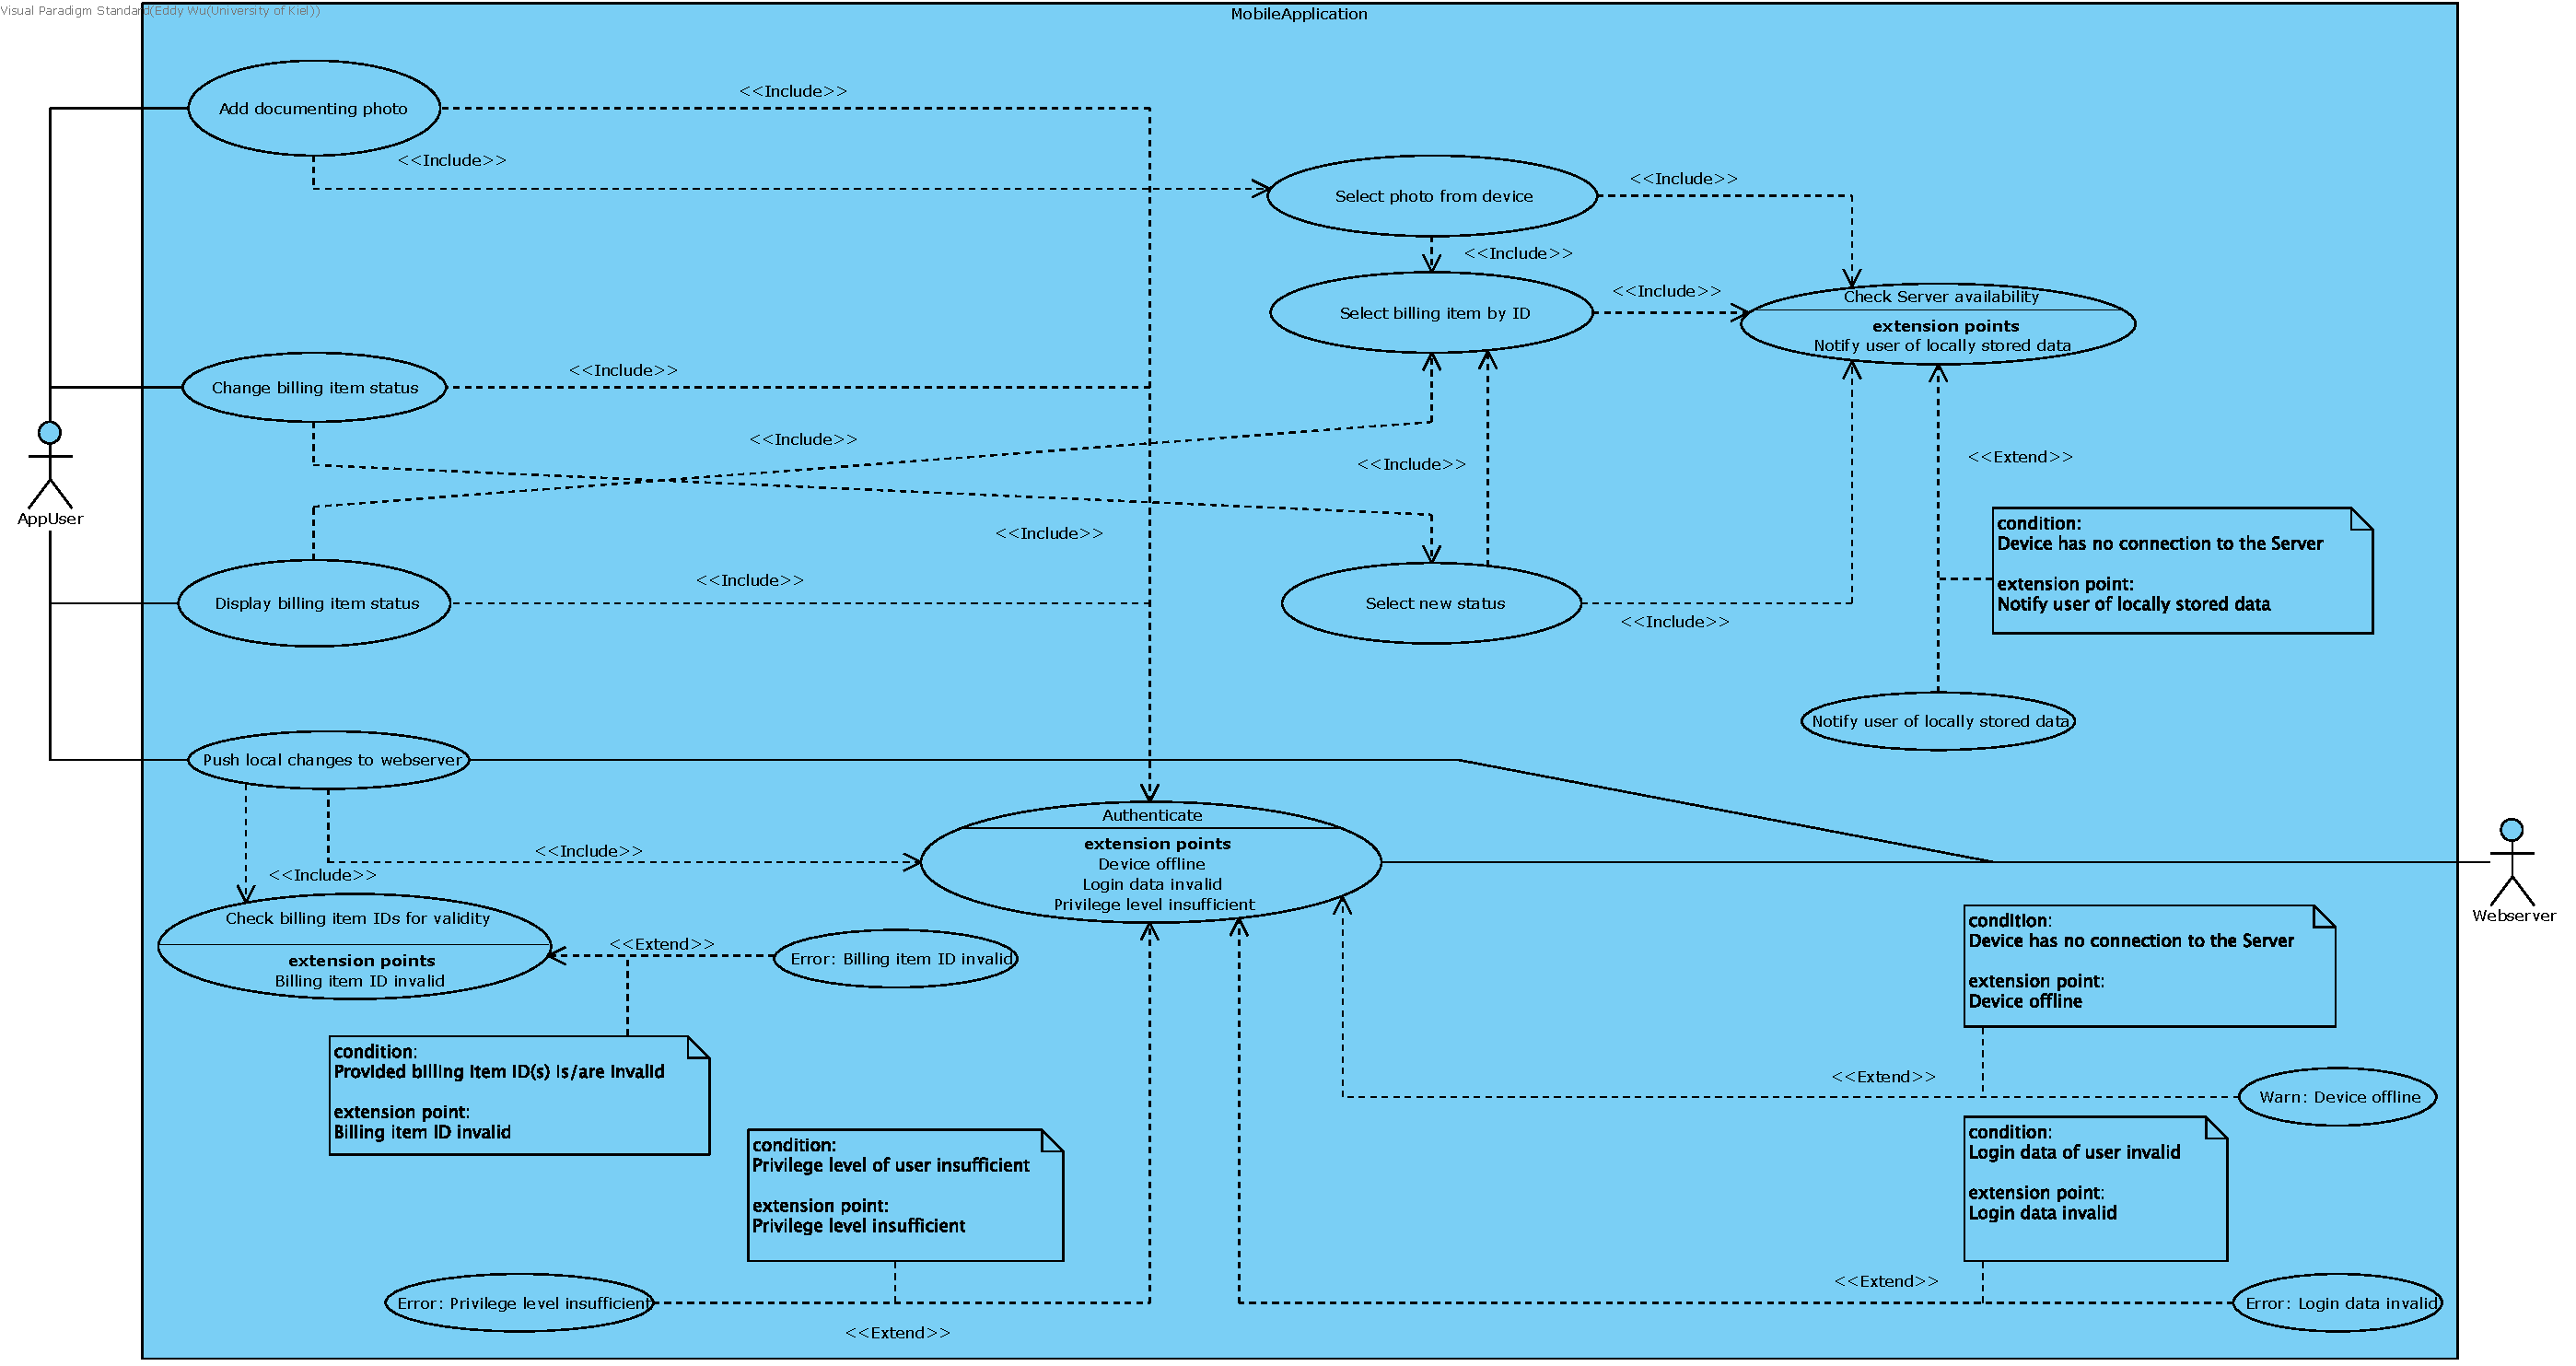
\includegraphics[width=\linewidth]{img/diagrams/Mobile_Application.pdf}
    \caption{Anwendungsfalldiagramm - App}
    \label{fig:anwendungsfalldiagramm-app}
\end{figure}
\centering
\begin{longtable}[c]{|p{4cm}|p{10cm}|}
    \caption{Anwendungsfall APP-1}
    \label{fig:anwendungsfall-app-tabelle-APP-1-4}
    \endlastfoot
    \hline \multicolumn{2}{|r|}{{Weitergeführt auf der folgenden Seite}}                                                                                                                                                                                                                                                                                           \\ \hline
    \endfoot
    \hline
    \endhead
    \hline
    \textbf{Anwendungsfall ID}          & APP-1                                                                                                                                                                                                                                                                                                                    \\ \hline
    \textbf{Anwendungsfallnamen}        & Change billing item status, Add documenting photo                                                                                                                                                                                                                                                                        \\ \hline
    \textbf{Initiierender Akteur}       & AppUser                                                                                                                                                                                                                                                                                                                  \\ \hline
    \textbf{Weitere Akteure}            & WebServer                                                                                                                                                                                                                                                                                                                \\ \hline
    \textbf{Kurzbeschreibung}           & Der Benutzer (AppUser) der Applikation kann lokale \"Anderungen,  bspw. \"Anderungen zum Baustatus einzelner Leistungspositionen oder Fotos mit Kommentar von der Baustelle, an den Webserver schicken. Diese \"Anderungen und Fotos mit Kommentar k\"onnen dann entsprechend \"uber die Webanwendung eingesehen werden. \\ \hline
    \textbf{Vorbedingungen}             & Der AppUser ist registriert und entsprechend eingeloggt                                                                                                                                                                                                                                                                  \\ \hline
    \textbf{Nachbedingungen}            & Die lokalen Daten wurden an den Webserver geschickt                                                                                                                                                                                                                                                                      \\ \hline
    \textbf{Ablauf}                     &
    \begin{enumerate}
        \item Der AppUser hat den Status einer Leistungsposition lokal ge\"andert.
        \item Der AppUser verwendet die Funktion der App,  um seine lokale \"Anderung an den Webserver zu \"ubertragen.
        \item Es besteht eine Internetverbindung und der AppUser erh\"alt die R\"uckmeldung, dass das Vorhaben erfolgreich ausgef\"uhrt wurde.
        \item Die \"Anderung befindet sich nun auf dem Webserver.
    \end{enumerate}                                                                                                                                                                                                                                                                                                                                      \\ \hline
    \textbf{Alternative}                &
    \begin{enumerate}
        \item Der AppUser hat seinen Benutzerrechten entsprechend ein Foto zur Dokumentation einer Leistungsposition angefertigt.
        \item Das Foto soll nun durch Bet\"atigen der entsprechenden Funktion der mobilen Applikation auf den Webserver hochgeladen werden.
        \item Es besteht eine Internetverbindung und der AppUser erh\"alt eine entsprechende Meldung,  dass der Upload erfolgt.
        \item Das Foto wird an den Webserver \"ubertragen.
    \end{enumerate}                                                                                                                                                                                                                                                                                                                                      \\ \hline
    \multirow{2}{*}{\textbf{Ausnahmen}} &
    \begin{enumerate}
        \item Der AppUser m\"ochte eine \"Anderung an dem Status einer Leistungsposition oder ein Foto zur Dokumentation mit Kommentar an den Webserver \"ubertragen und verwendet die entsprechende Funktionalit\"at der Applikation.
        \item Der AppUser erh\"alt eine Fehlermeldung, da seine Rechte nicht ausreichen, um diese Aktion durchzuf\"uhren.
        \item Die \"Anderungen am Status der Leistungsposition und/oder das Foto mit Kommentar werden nicht an den Webserver \"ubertragen.
    \end{enumerate}
    \\\cline{2-2}                 &
    \begin{enumerate}
        \item Die lokalen \"Anderungen durch den AppUser sollen durch Bet\"atigung der entsprechenden Funktion in der App an den Webserver \"ubertragen werden.
        \item Der AppUser erh\"alt eine Fehlermeldung, da zur Zeit f\"ur das verwendete Ger\"at keine (ausreichende) Internetverbindung besteht.
        \item Der AppUser erh\"alt eine R\"uckmeldung, dass zur Zeit keine Internetverbindung besteht und lokale \"Anderungen zwischengespeichert werden.
        \item Sobald eine ausreichende Internetverbindung besteht, werden die entsprechenden Daten an den Webserver \"ubertragen.
    \end{enumerate}
    \\\cline{2-2}                 &
    \begin{enumerate}
        \item Der AppUser m\"ochte eine lokale \"Anderung an dem Status einer Leistungsposition oder ein Foto mit Kommentar an den Webserver \"ubertragen und verwendet die entsprechende Funktion in der Applikation.
        \item Die Identifikationsnummer der betroffenen Leistungsposition ist nicht g\"ultig.
        \item Der AppUser erh\"alt eine Fehlermeldung.
        \item Die \"Anderungen am Status der Leistungsposition oder das Foto mit Kommentar werden nicht an den Webserver \"ubertragen.
    \end{enumerate}                                                                                                                                                                                                                                                                                                                                     \\ \hline
    \textbf{Benutzte Anwendungsfälle}   & Benutzerverwaltung (ACC-1)                                                                                                                                                                                                                                                                                               \\ \hline
    \textbf{Spezielle Anforderungen}    & -                                                                                                                                                                                                                                                                                                                        \\ \hline
    \textbf{Annahmen}                   & -                                                                                                                                                                                                                                                                                                                        \\ \hline
\end{longtable}

\clearpage

\section{Anwendungsfalldiagramme - Webserver}

\subsection{Account-Management}

\begin{figure}[h]
    \centering
    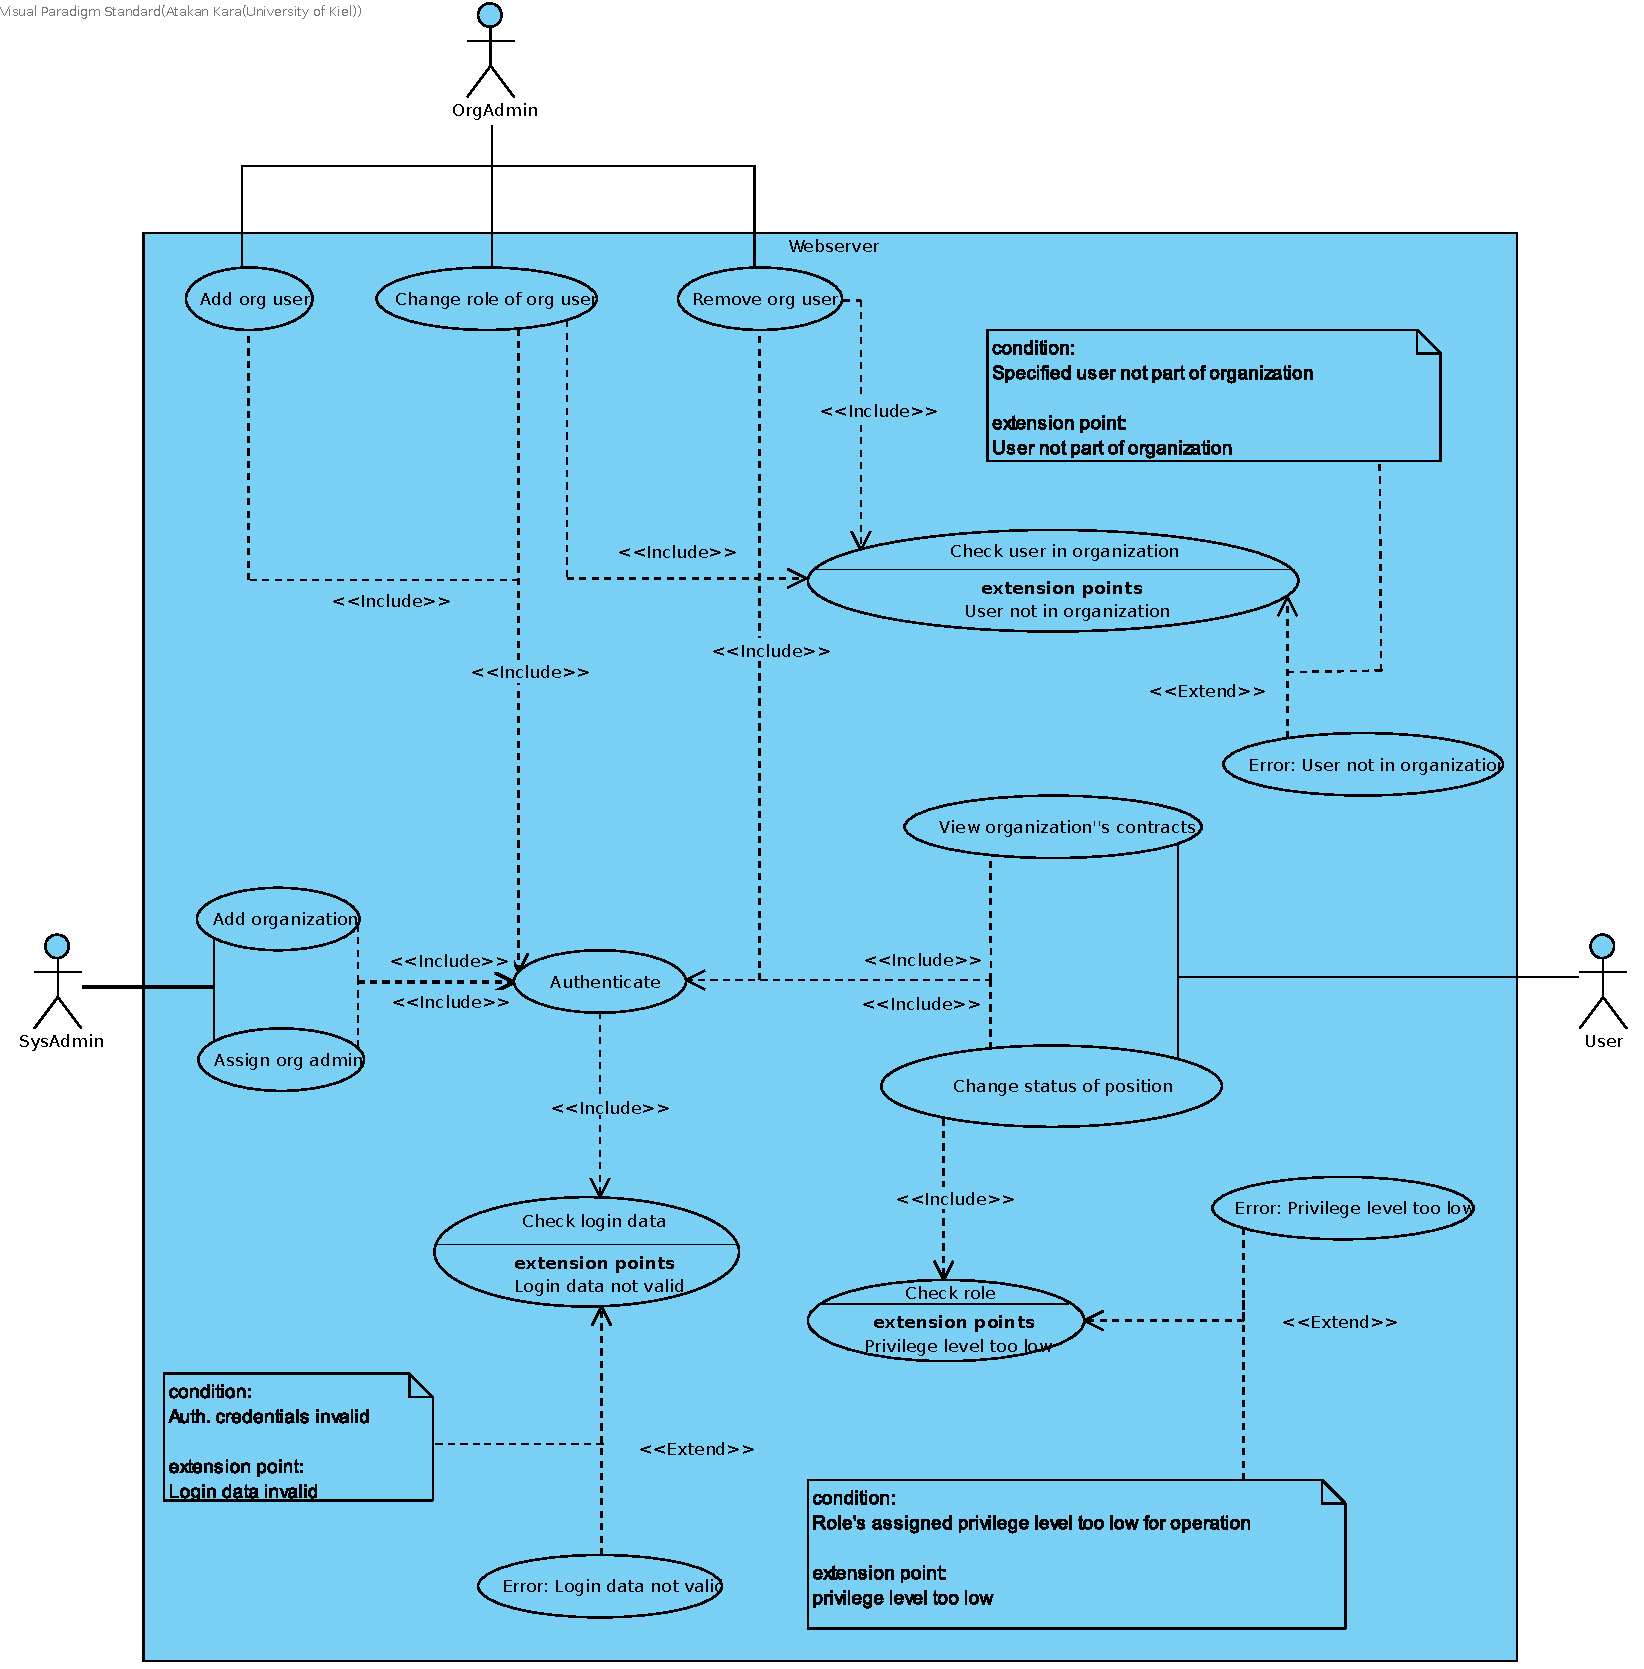
\includegraphics[width=\linewidth]{img/diagrams/Acc_Management_Web.pdf}
    \caption{Anwendungsfalldiagramm - Account-Management Webserver}
    \label{fig:anwendungsfalldiagramm-acc}
\end{figure}

Das Hinzufügen, Editieren und Löschen von Nutzern sowie Organisationen wird als trivial erachtet und im Folgenden nicht näher betrachtet. Selbiges gilt für die Einsicht von Verträgen einer Organisation.

\centering
\begin{longtable}[c]{|p{4cm}|p{10cm}|}
    \caption{Anwendungsfall ACC-1}
    \label{fig:anwendungsfall-server-tabelle-ACC-1}
    \endlastfoot
    \hline \multicolumn{2}{|r|}{{Weitergeführt auf der folgenden Seite}}                                                                   \\ \hline
    \endfoot
    \hline
    \endhead
    \hline
    \textbf{Anwendungsfall ID}        & ACC-1                                                                                              \\ \hline
    \textbf{Anwendungsfallname}       & Change status of position                                                                          \\ \hline
    \textbf{Initiierender Akteur}     & WebUser                                                                                            \\ \hline
    \textbf{Weitere Akteure}          & -                                                                                                  \\ \hline
    \textbf{Kurzbeschreibung}         & Der WebUser kann den Status von Leistungspositionen ver\"andern                                    \\ \hline
    \textbf{Vorbedingungen}           & Der WebUser ist entsprechend eingeloggt, Rechte des WebUser sind ausreichend f\"ur diese Operation \\ \hline
    \textbf{Nachbedingungen}          & Status wurde ver\"andert                                                                           \\ \hline
    \textbf{Ablauf}                   &
    \begin{enumerate}
        \item Der WebUser \"andert den Status einer Leistungsposition und w\"ahlt die entsprechende Funktion der Weboberfl\"ache, dass diese \"Anderung \"ubernommen werden soll.
        \item Die Aktion war erfolgreich und die \"Anderung wurde \"ubernommen.  Der User erh\"alt eine R\"uckmeldung \"uber den Erfolg der Aktion.
    \end{enumerate}                                                                                                             \\ \hline
    \textbf{Alternative}              & -
    \\ \hline
    \textbf{Ausnahme}                 &
    \begin{enumerate}
        \item Der WebUser \"andert den Status einer Leistungsposition und w\"ahlt die entsprechende Funktion der Weboberfl\"ache,  dass diese \"Anderung \"ubernommen werden soll.
        \item Der WebUser verf\"ugt nicht \"uber die entsprechenden Rechte die Aktion durchzuf\"uhren und erh\"alt eine Fehlermeldung. Der bisherige Status der Leistungsposition bleibt bestehen.
    \end{enumerate}                                                                                                             \\ \hline
    \textbf{Benutzte Anwendungsfälle} & -                                                                         \\ \hline
    \textbf{Spezielle Anforderungen}  & -                                                                                                  \\ \hline
    \textbf{Annahmen}                 & -                                                                                                  \\ \hline
\end{longtable}

\clearpage

\subsection{Diagrammdarstellung}

\begin{figure}[h]
	\centering
	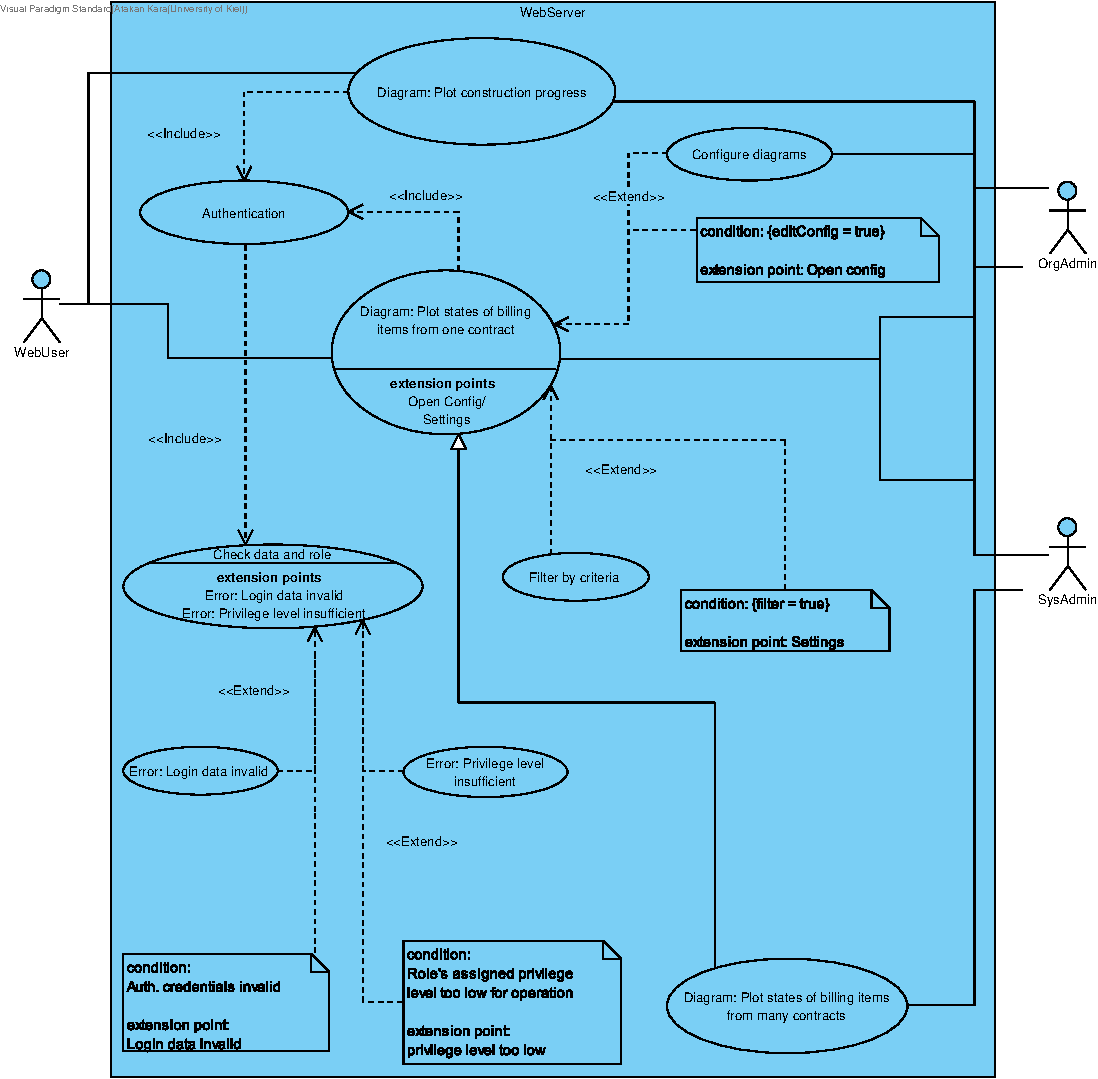
\includegraphics[width=\linewidth]{img/diagrams/Manage_Diagrams.pdf}
	%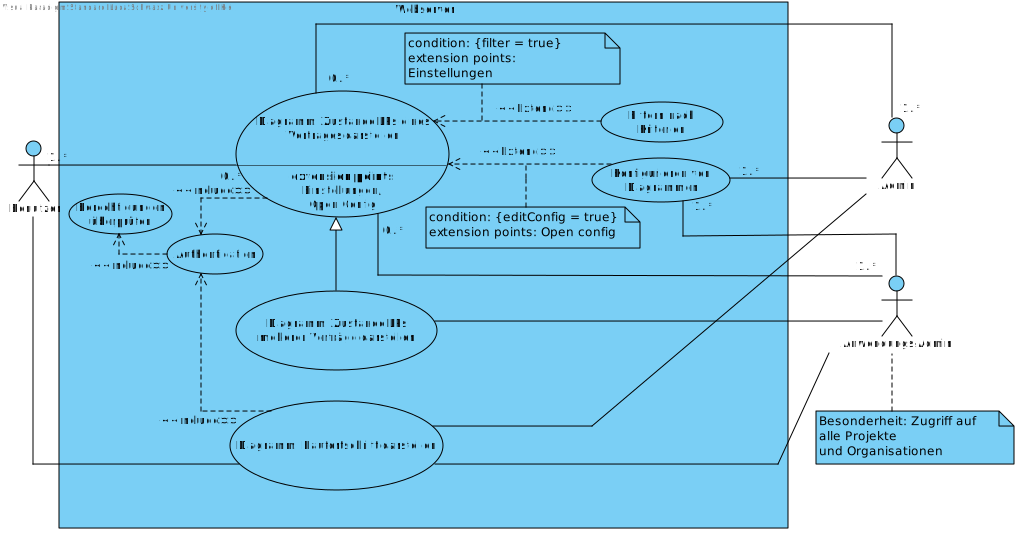
\includegraphics[width=\linewidth]{img/diagrams/Diagram_Display_Management_Web.svg}
	\caption{Anwendungsfalldiagramm - Diagrammdarstellung}
	\label{fig:anwendungsfalldiagramm-dia-verwaltung}
\end{figure}

\centering
\begin{longtable}[c]{|p{4cm}|p{10cm}|}
    \caption{Anwendungsfall DIA-1}
    \label{fig:anwendungsfall-diagrammdarstellung-tabelle-DIA-1}
    \endlastfoot
    \hline \multicolumn{2}{|r|}{{Weitergeführt auf der folgenden Seite}}                                                                                     \\ \hline
    \endfoot
    \hline
    \endhead
    \hline
    \textbf{Anwendungsfall ID}             & DIA-1                                                                                                           \\ \hline
    \textbf{Anwendungsfallnamen}           & Diagramm: Plot construction progress, Diagram: Plot states of billing items from one contract                   \\ \hline
    \textbf{Initiierender Akteur}          & WebUser                                                                                                         \\ \hline
    \textbf{Weitere Akteure}               & SysAdmin, OrgAdmin                                                                                              \\ \hline
    \textbf{Kurzbeschreibung}              & Darstellung und mögliche Filterung der vom Server automatisch erzeugten Diagramme innerhalb der Webapplikation. \\ \hline
    \textbf{Vorbedingungen}                & Funktionierende Internetverbindung, bestätigte Berechtigungen (Authentifiziert)                                 \\ \hline
    \textbf{Nachbedingungen}               & -                                                                                                               \\ \hline
    \textbf{Ablauf}                        &
    \begin{enumerate}
        %\item Erfolgreich authentifizieren (passende Rolle).
        \item Der WebUser authentifiziert sich (passende Rolle).
        \item Der WebUser wechselt in den Reiter der Diagramme.
              %\item Darstellen eines allgemeinen (alle Leistungspunkte umfassend) Diagramms zu einem oder mehreren Verträgen.
        \item Der WebUser wählt ein alle Leistungspunkte umfassendes Diagramm eines oder mehrere Verträge zur Darstellung.
        \item Das Diagramm wird angezeigt.
    \end{enumerate}                                                                                                                               \\ \hline
    \multirow{2}{*}{\textbf{Alternativen}} &
    %%\textbf{Alternative} &
    \begin{enumerate}
        %\item Erfolgreich authentifizieren (passende Rolle).
        \item Der WebUser authentifiziert sich (passende Rolle).
        \item Der WebUser wechselt in den Reiter der Diagramme.
        \item Der WebUser filtert nach bestimmten Kriterien.
              %\item Darstellen eines Diagramms zu einem oder mehreren Verträgen.
        \item Das Diagramm wird angezeigt.
    \end{enumerate}                                                                                                                               \\\cline{2-2} &
    \begin{enumerate}
        %\item Erfolgreich authentifizieren (passende Rolle).
        \item Der WebUser authentifiziert sich (passende Rolle).
        \item Der WebUser wechselt in den Reiter der Diagramme.
        \item Der WebUser wählt das Diagramm zum Baufortschritt eines Projektes.
        \item Das Diagramm wird angezeigt.
    \end{enumerate}                                                                                                                               \\ \hline
    \multirow{2}{*}{\textbf{Ausnahmen}}    &
    \begin{enumerate} % Projekt/Vertrag nicht vorhanden.
        %\item Erfolgreich authentifizieren (passende Rolle).
        \item Der WebUser authentifiziert sich (passende Rolle).
        \item Der WebUser wechselt in den Reiter der Diagramme.
        \item Der WebUser wählt ein nicht-existentes Projekt aus.
        \item Fehlermeldung!
    \end{enumerate}                                                                                                                               \\\cline{2-2} &
    \begin{enumerate} % Kriterien werden nicht erfüllt.
        \item Der WebUser authentifiziert sich (passende Rolle).
        \item Der WebUser wechselt in den Reiter der Diagramme.
        \item Der WebUser filtert nach bestimmten Kriterien.
        \item Die Kriterien werden von keinem Diagramm erfüllt.
        \item Fehlermeldung!
    \end{enumerate}                                                                                                                               \\\cline{2-2} &
    \begin{enumerate} % Fehlende Berechtigungen.
        %\item Erfolgreich authentifizieren (\textbf{keine} passende Rolle).
        \item Der WebUser authentifiziert sich (\textbf{keine} passende Rolle).
        \item Der WebUser wechselt in den Reiter der Diagramme.
              %\item Diagramm ohne passende Rolle anzeigen lassen.
        \item Der WebUser wählt ein Diagramm, für welches er keine Rechte hat.
        \item Fehlermeldung!
    \end{enumerate}                                                                                                                               \\\cline{2-2} &
    \begin{enumerate} % Fehlende Berechtigungen für einzelne LPs.
        %\item Erfolgreich authentifizieren (\textbf{keine} passende Rolle).
        \item Der WebUser authentifiziert sich (\textbf{keine} passende Rolle).
        \item Der WebUser wechselt in den Reiter der Diagramme.
              %\item Diagramm ohne passende Rolle anzeigen lassen.
        \item Der WebUser filtert nach bestimmten Kriterien, wofür er keine Rechte hat.
        \item Fehlermeldung!
    \end{enumerate}                                                                                                                               \\ \hline
    \textbf{Benutzte Anwendungsfälle}      & Benutzerverwaltung (ACC-1)                                                                                      \\ \hline
    \textbf{Spezielle Anforderungen}       & -                                                                                                               \\ \hline
    \textbf{Annahmen}                      & -                                                                                                               \\ \hline
\end{longtable}

\clearpage

\subsection{Diagrammerstellung}

\begin{figure}[h]
    \centering
    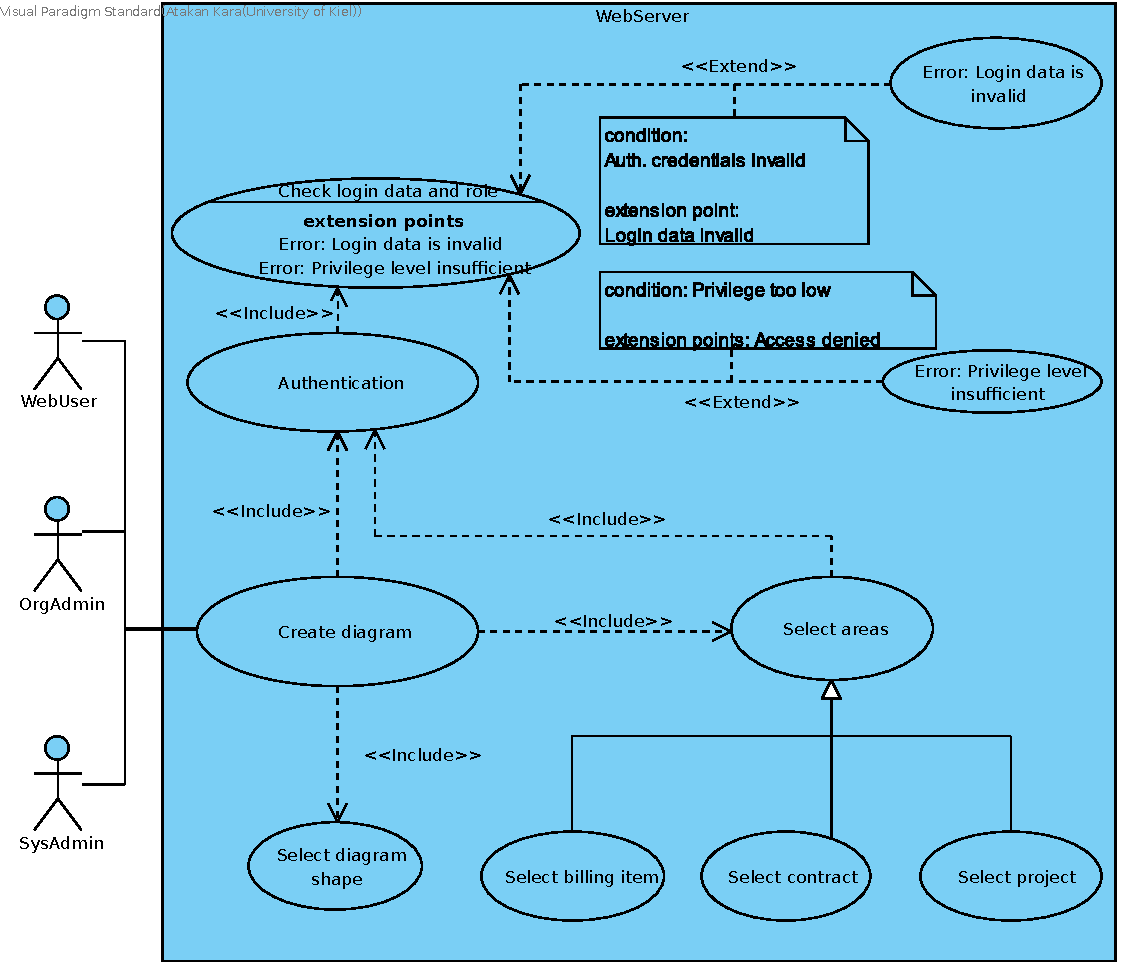
\includegraphics[width=\linewidth]{img/diagrams/Create_Custom_Diagram.pdf}
    \caption{Anwendungsfalldiagramm - Diagrammerstellung}
    \label{fig:anwendungsfalldiagramm-dia-erstellung}
\end{figure}

\centering
\begin{longtable}[c]{|p{4cm}|p{10cm}|}
    \caption{Anwendungsfall DIA-2}
    \label{fig:anwendungsfall-DIA-2}
    \endlastfoot
    \hline \multicolumn{2}{|r|}{{Weitergeführt auf der folgenden Seite}}                                                                                                                                                                                       \\ \hline
    \endfoot
    \hline
    \endhead
    \hline
    \textbf{Anwendungsfall ID}          & DIA-2                                                                                                                                                                                                                \\ \hline
    \textbf{Anwendungsfallname}         & Create diagram                                                                                                                                                                                                       \\ \hline
    \textbf{Initiierender Akteur}       & WebUser, SysAdmin, OrgAdmin                                                                                                                                                                                          \\ \hline
    \textbf{Kurzbeschreibung}           & Nutzer der Weboberfläche (allgemein WebUser) können aus den für sie lesbaren Daten auf dem Server, aus den Bereichen Leistungsposition, Vertrag und Projekt, Diagramme in unterschiedlichen Darstellungen erstellen. \\ \hline
    \textbf{Vorbedingungen}             & Der WebUser hat Zugriffsrechte auf die zu visualisierenden Daten.                                                                                                                                                    \\ \hline
    \textbf{Nachbedingungen}            & Dem WebUser wird das angefragte Diagramm angezeigt.                                                                                                                                                                  \\ \hline
    \textbf{Ablauf}                     &
    \begin{enumerate}
        \item Der WebUser loggt sich in der Weboberfläche mit den Benutzerdaten, bestehend aus Benutzername und Passwort, ein.
        \item Der WebUser wählt eine Diagramm-Darstellung .
        \item Der WebUser wählt aus einer Liste Leistungspositionen, Verträge und Projekte aus, auf die er Zugriff hat und die er im Diagramm visualisieren möchte.
        \item Es wird eine Anfrage an den Server bezüglich der Übermittlung der Daten geschickt.
        \item Das Diagramm wird dem WebUser angezeigt.
    \end{enumerate}                                                                                                                                                                                                                                 \\ \hline

    \textbf{Alternative}                & -                                                                                                                                                                                                                    \\ \hline

    \multirow{2}{*}{\textbf{Ausnahmen}} &
    \begin{enumerate} % Nutzer wählt Daten aus ohne Zugriffsrecht / während der Bereich-auswahl
        \item Der WebUser loggt sich in der Weboberfläche mit den Benutzerdaten, bestehend aus Benutzername und Passwort, ein.
        \item Der WebUser wählt eine Diagramm-Darstellung.
        \item Der WebUser wählt aus einer Liste Leistungspositionen, Verträge und Projekte aus, auf die er Zugriff hat und die er im Diagramm visualisieren möchte.
        \item Es wird eine Anfrage an den Server bezüglich der Übermittlung der Daten geschickt.
        \item Der Server verweigert den Zugriff auf die Daten durch fehlende Zugriffsrechte.
    \end{enumerate}                                                                                                                                                                                                                                 \\\cline{2-2} &
    \begin{enumerate} % Verbindungsfehler
        \item Der WebUser loggt sich in der Weboberfläche mit den Benutzerdaten, bestehend aus Benutzername und Passwort, ein.
        \item Der WebUser wählt eine Diagramm-Darstellung .
        \item Der WebUser wählt aus einer Liste Leistungspositionen, Verträge und Projekte aus, auf die er Zugriff hat und die er im Diagramm visualisieren möchte.
        \item Es wird eine Anfrage an den Server bezüglich der Übermittlung der Daten geschickt.
        \item Verbindungsfehler
    \end{enumerate}                                                                                                                                                                                                                                 \\ \hline
    \textbf{Benutzte Anwendungsfälle}   & Benutzerverwaltung (ACC-1), Diagrammverwaltung (DIA-1)                                                                                                                                                               \\ \hline
    \textbf{Spezielle Anforderungen}    & -                                                                                                                                                                                                                    \\ \hline
    \textbf{Annahmen}                   & -                                                                                                                                                                                                                    \\ \hline
\end{longtable}